% A good introduction to latex can be found here:
%  http://www.cse.ohio-state.edu/~hank/latex/lshort141.pdf

\documentclass{article}
\usepackage{graphicx}
\usepackage{full page}  % make the margins somewhat smaller than the default

\usepackage{listings}  %  needed for source code listings
\lstset{language=Java}

% set the document title, author, and date here.
%  once set, the \maketitle command (within the document)
%  will display them nicely
\title{Missionaries and Cannibals Solution}
\author{Seyed Mahdi Basiri Azad (Erfan)}

\begin{document}
\maketitle

\section{Introduction}
Missionaries and Cannibals is a game in which the objective is to transfer a group of missionaries and a group of cannibals from one side of the river to the other using a single boat \verb`safely`. The boat will have a fixed capacity (2, in the standard <3,3,1> game). The main constraint is that if the number of cannibals becomes higher than the number of missionaries on either side of the river the missionaries of that side will be eaten. The upper bound for the number of states in this game would be 4*4*2=32 because in <M,C,B> M and C can take values of 0 to 3 and the B can be a 1 or a 0.


In order to find the solution to this game we created a model for the game with states representing the condition of the game at each point. The states where then wrapped in nodes and connected to each other to form a tree. By finding a path from the starting node to the goal node we will find the solution path. Hence the game is reduced to a simple tree search among the possible states.


In order to implement the game, we created a Model-Controller system. The \verb`cannibalProblem.java` would create the model holding the information about the game and each state in its \verb`cannibalNode` class and the \verb`UUSearchProblem.java` would contain the different search algorithms to solve the problem.


We used a variety of search algorithms for this problem including:
\begin{itemize}
\item Breadth First Search
\item Depth First Memoizing Search
\item Depth First Path Checking Search
\item Iterative Deepening Search
\end{itemize}



\section{Implementation of the model}

The model is implemented in
\verb`CannibalProblem.java`. The model extends the UUSearchProblem class and holds information about the problem itself, such as the number of Missionaries and Cannibals, and also implements the UUSearchNode interface to be used as a wrapper class for the states of the game. The Most important part of cannibalNode class is the \verb`getSuccessors()` function. This function creates the children/successors of the current cannibalNode which are all the nodes that can be reached from that cannibalNode. In order to implement it I created two helper functions called:
\begin{enumerate}
\item \verb`isFeasibleState(int[] state)`
\item \verb`isLegalState(int[] state)`
\end{enumerate}

Given a boat with capacity of 2, there are maximum of 5 actions that can take place from each state. So in the \verb`getSuccessors()` I first created all the "Possible" successors then I passed those nodes through the two helper functions to filter out the ones that were not feasible, such as taking two cannibals from a side of the shore which only has one cannibal, and the ones that were not legal, meaning that they would lead to the death of the missionaries. I then return a list of successor nodes after the filtering.
Here's my code for \verb`getSuccessors`:

\begin{lstlisting}
public ArrayList<UUSearchNode> getSuccessors() {
  ArrayList<UUSearchNode> successors = new ArrayList<UUSearchNode>();
  ArrayList<CannibalNode> helper = new ArrayList<CannibalNode>();

  if (this.state[2]==1){ //if the boat is on the starting shore
   helper.add(new CannibalNode(this.state[0] - 2, this.state[1],
  this.state[2] - 1, this.depth + 1)); //subtracting <201>
   helper.add(new CannibalNode(this.state[0], this.state[1] - 2,
  this.state[2] - 1, this.depth + 1)); //subtracting <021>
   helper.add(new CannibalNode(this.state[0] - 1, this.state[1] - 1,
  this.state[2] - 1, this.depth + 1)); //subtracting <111>
   helper.add(new CannibalNode(this.state[0] - 1, this.state[1],
  this.state[2] - 1, this.depth + 1)); //subtracting <101>
   helper.add(new CannibalNode(this.state[0], this.state[1] - 1,
  this.state[2] - 1, this.depth + 1)); //subtracting <011>
  }else{ //if the boat is on the opposite shore
   helper.add(new CannibalNode(this.state[0] + 2, this.state[1],
  this.state[2] + 1, this.depth + 1)); //adding <201>
   helper.add(new CannibalNode(this.state[0], this.state[1] + 2,
  this.state[2] + 1, this.depth + 1)); //adding <021>
   helper.add(new CannibalNode(this.state[0] + 1, this.state[1] + 1,
  this.state[2] + 1, this.depth + 1)); //adding <111>
   helper.add(new CannibalNode(this.state[0] + 1, this.state[1],
  this.state[2] + 1, this.depth + 1)); //adding <101>
   helper.add(new CannibalNode(this.state[0], this.state[1] + 1,
  this.state[2] + 1, this.depth + 1)); //adding <011>
  }
  //now we check for feasibility and legality
  for(CannibalNode n : helper){
   if(isFeasibleState(n.state) && isLegalState(n.state)){
  successors.add(n);
   }
  }
  return successors;
 }
\end{lstlisting}


And below are my \verb`isFeasibleState(int[] state)` and \verb`isLegalState(int[] state)` functions:


\begin{lstlisting}
private boolean isFeasibleState(int[] state){
  if((state[0] <= totalMissionaries && state[0] >= 0)&&
  (state[1] <= totalCannibals && state[1] >= 0)) {
   return true;}return false;}
\end{lstlisting}

\begin{lstlisting}
private boolean isLegalState(int[] state){
  int[] stateOtherSide = new int[3];
  stateOtherSide[0] = totalMissionaries - state[0];
  stateOtherSide[1] = totalCannibals - state[1];
  stateOtherSide[2] = state[2]==0 ? 1 : 0;
  if((state[0] < state[1]) && state[0] >0 ||
  (stateOtherSide[0] < stateOtherSide[1]) && stateOtherSide[0] > 0) {
  	return false;}else{return true;}}
\end{lstlisting}
\break
The graph below shows the first two levels of the graph for starting state of <3,3,1>. The nodes are all expanded for the startNode (including the not legal ones).


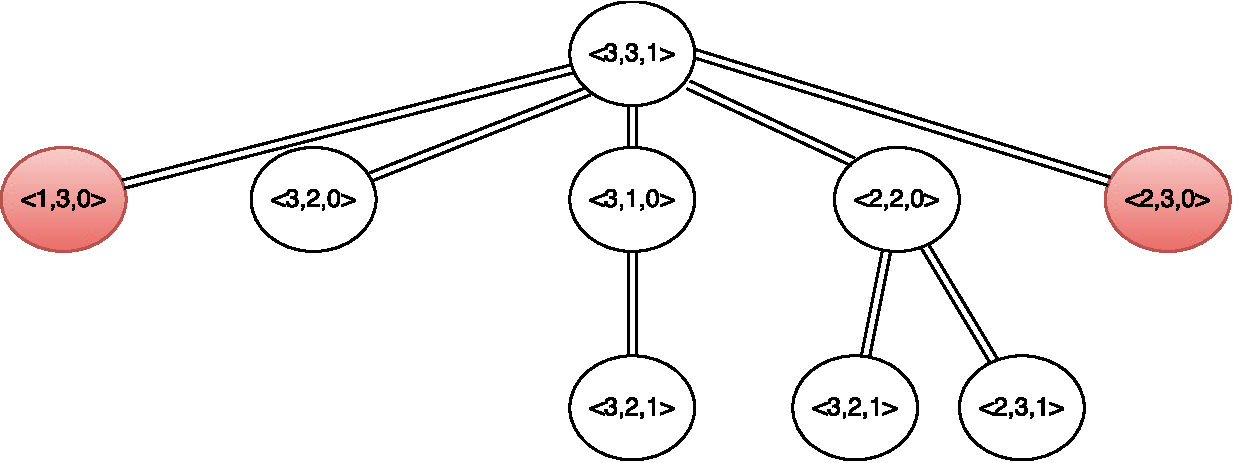
\includegraphics[scale=0.75]{states2}

\section{Breadth-first search}
For the Breadth First Search I used java's LinkedList class to implement a Queue as the frontier to hold the nodes that are to be visited.
I used a HashSet to mark all the visited nodes and used a HashMap called "relations" to hold the nodes and their parents as the children are created. I opted to separate the Explored HashSet from Relation HashMap because I would want to add the Nodes to the Explored set after they are out of the Queue however at that point there might not be any sign of their parents.
Below is the major portion of BFS after checking if the startNode is the goal node:
\begin{lstlisting}
...
else{ //start searching
  frontier.add(startNode);
  relations.put(startNode, null);
  while(!frontier.isEmpty()){
  UUSearchNode n = frontier.poll();//pop
  explored.add(n);
  List<UUSearchNode> children = n.getSuccessors(); //get children
  for(UUSearchNode child: children){
    if(!explored.contains(child) && !frontier.contains(child)){
  if(child.goalTest()){
  	  relations.put(child,n);
  return backchain(child, relations);
  }
  relations.put(child, n);
  frontier.add(child);
    }
  }
  }
  return null; // failure to find the goal (goal does not exist!)
 }
\end{lstlisting}

The \verb`backchain()` function simple follows the given node back to the startNode given the "relation" HashMap and creates a List of nodes along the way and returns it.

\section{Memoizing depth-first search}
We used recursion to write the Memoizing-DFS. There were two base-cases for the recursions that were used for all kinds of recursive DFS algorithms used in this project:
\begin{enumerate}
\item Goal node has been reached
\item Maximum Depth has exceeded
\end{enumerate}
If the goal node was found then an List will be initialized with the goal node in it ans will be returned to the caller which then will add the parent (caller) node to the List and pass it on and so forth.
Below is the core of the Memoizing-DFS notice that it holds all the visited nodes in a HashSet, which increases the memory usage of the DFS which was main good thing about DFS.
\begin{lstlisting}
  List<UUSearchNode> path = null;
  visited.add(currentNode); //mark the current node as visited
  if(currentNode.goalTest()){ //if the current node is the goal (basecase 1)
    path = new ArrayList<UUSearchNode>();
    path.add(currentNode);
    return path;
  }else if(depth > maxDepth){ //if we have reached the cutoff depth (basecase 2)
    System.out.println("Exceeded Maximum depth of " + maxDepth + " with NO RESULT");
    return null;
  }else{ // (recursive case)
    ArrayList<UUSearchNode> children = currentNode.getSuccessors(); //get children
    for (UUSearchNode child : children){
      if(!visited.contains(child)) {// if not yet visited then visit it!
        path = dfsrm(child, visited, depth + 1, maxDepth); //(Here be recursion!)
        if(path != null) {// not failure or cutoff
          //we have found the goal, add currentNode to the path and pass it on!
          path.add(currentNode);
          return path;
        }
      }
    }
    return null; // failure
  }
\end{lstlisting}

\section{Path-checking depth-first search}
The Only major difference between Path-Checking-DFS and Memoizing-DFS is that in Path-Checking-DFS we won't keep track of all the visited nodes but only the ones that are part of the current path, this way we can avoid loops as well as keep the desired memory efficiency of the DFS algorithm.

\section{Iterative deepening search}
Iterative deepening has the Path-Checking-DFS at its core however it increments the maximum depth of the search in each iteration. It is as if we were doing the BFS however it is more memory efficient but there is a trade off because Iterative-Deepening runs the Path-Checking-DFS from scratch in every iteration.

\section{Search Results and comparison}
After running the programs with startNode of <8,5,1> we could clearly see the difference between in memory usage between different searches. Iterative-Deepening-DFS use the least amount of memory however it was clearly the slowest one given that its number of nodes explored was 4 orders of magnitude higher than of the others. Below are the results from runing the \verb`CannibalDriver.java`
\begin{lstlisting}
bfs path length:  24
Nodes explored during last search:  57
Maximum memory usage during last search 56
--------
dfs memoizing path length:46
Nodes explored during last search:  56
Maximum memory usage during last search 55
--------
dfs path checking path length:46
Nodes explored during last search:  56
Maximum memory usage during last search 45
--------
Iterative deepening (path checking) path length:24
Nodes explored during last search:  246678
Maximum memory usage during last search 23
\end{lstlisting}



\section{Lossy missionaries and cannibals}
In implementing a lossy version of this game, such that E number of Missionaries could be eaten during the game the main change would be in the \verb`getSuccessors()` method. more specifically the change will be in the \verb`isLegalState()`. There will also be a global counter in the problem that will count the number of missionaries that have been eaten against the number of Missionaries that can possibly be eaten, E.




\end{document}